\chapter{Optimalizace}
	
\section{Postup optimalizace}
	Před tím, než přistoupíme k problému optimalizace, je třeba získat potřebná data. Důležité jsou informace o parametrech svazků, které lze rozdělit na \textit{simulované} a \textit{reálné}.

\subsection*{Simulované svazky}
\begin{enumerate}

\item 	Nejprve potřebné potřebné parametry kamene, který zkoumáme. Zdrojem může být technický výkres, nebo předchozí měření.  

\item	Sestavíme model, který bude přibližně určovat tvar kamene. Tento model budeme považovat za \textit{referenční}.

\item	V programu LADOK simulujeme průlet svazku \textit{referenčním} modelem. Pro simulaci je důležité znát elektromagnetické vlastnosti laserového svazku a přibližný index lomu kamene. 

\item	Výsledkem simulace jsou parametry \textit{simulovaných} svazků.

\end{enumerate}

\subsection*{Reálné svazky}
Předpokladem pro získání parametrů \textit{reálných} svazků je sestavení a kalibrace měřicí soustavy podle \cite{Drapela}. 
\begin{enumerate}

\item 	Opracovaný kámen umístíme do měřicí soustavy.

\item	Provedeme experiment průchodu svazku kamenem podobný situaci v simulačním programu LADOK. 

\item	Získáme obraz dopadu laserových svazků na stínítko. 

\item	V obraze detekujeme světelné stopy (kapitola \ref{sec:detection}).  

\item	Z detekovaných stop vypočítáme parametry \textit{reálných} svazků (kapitola \ref{sec:beam parameters}).

\end{enumerate}

Přecházíme k situaci, kdy máme dostupné informace o simulovaných i reálných svazcích. Mezi těmito dvěma množinami je třeba nalézt korespondence. Korespondující svazky si odpovídají seznamem faset kamene, na které při své cestě dopadají.  


% diagram je vytvoren -> 500pm -> bitmap -> online to EPS -> latex to PDF -> load PDF
\begin{figure}
\centering
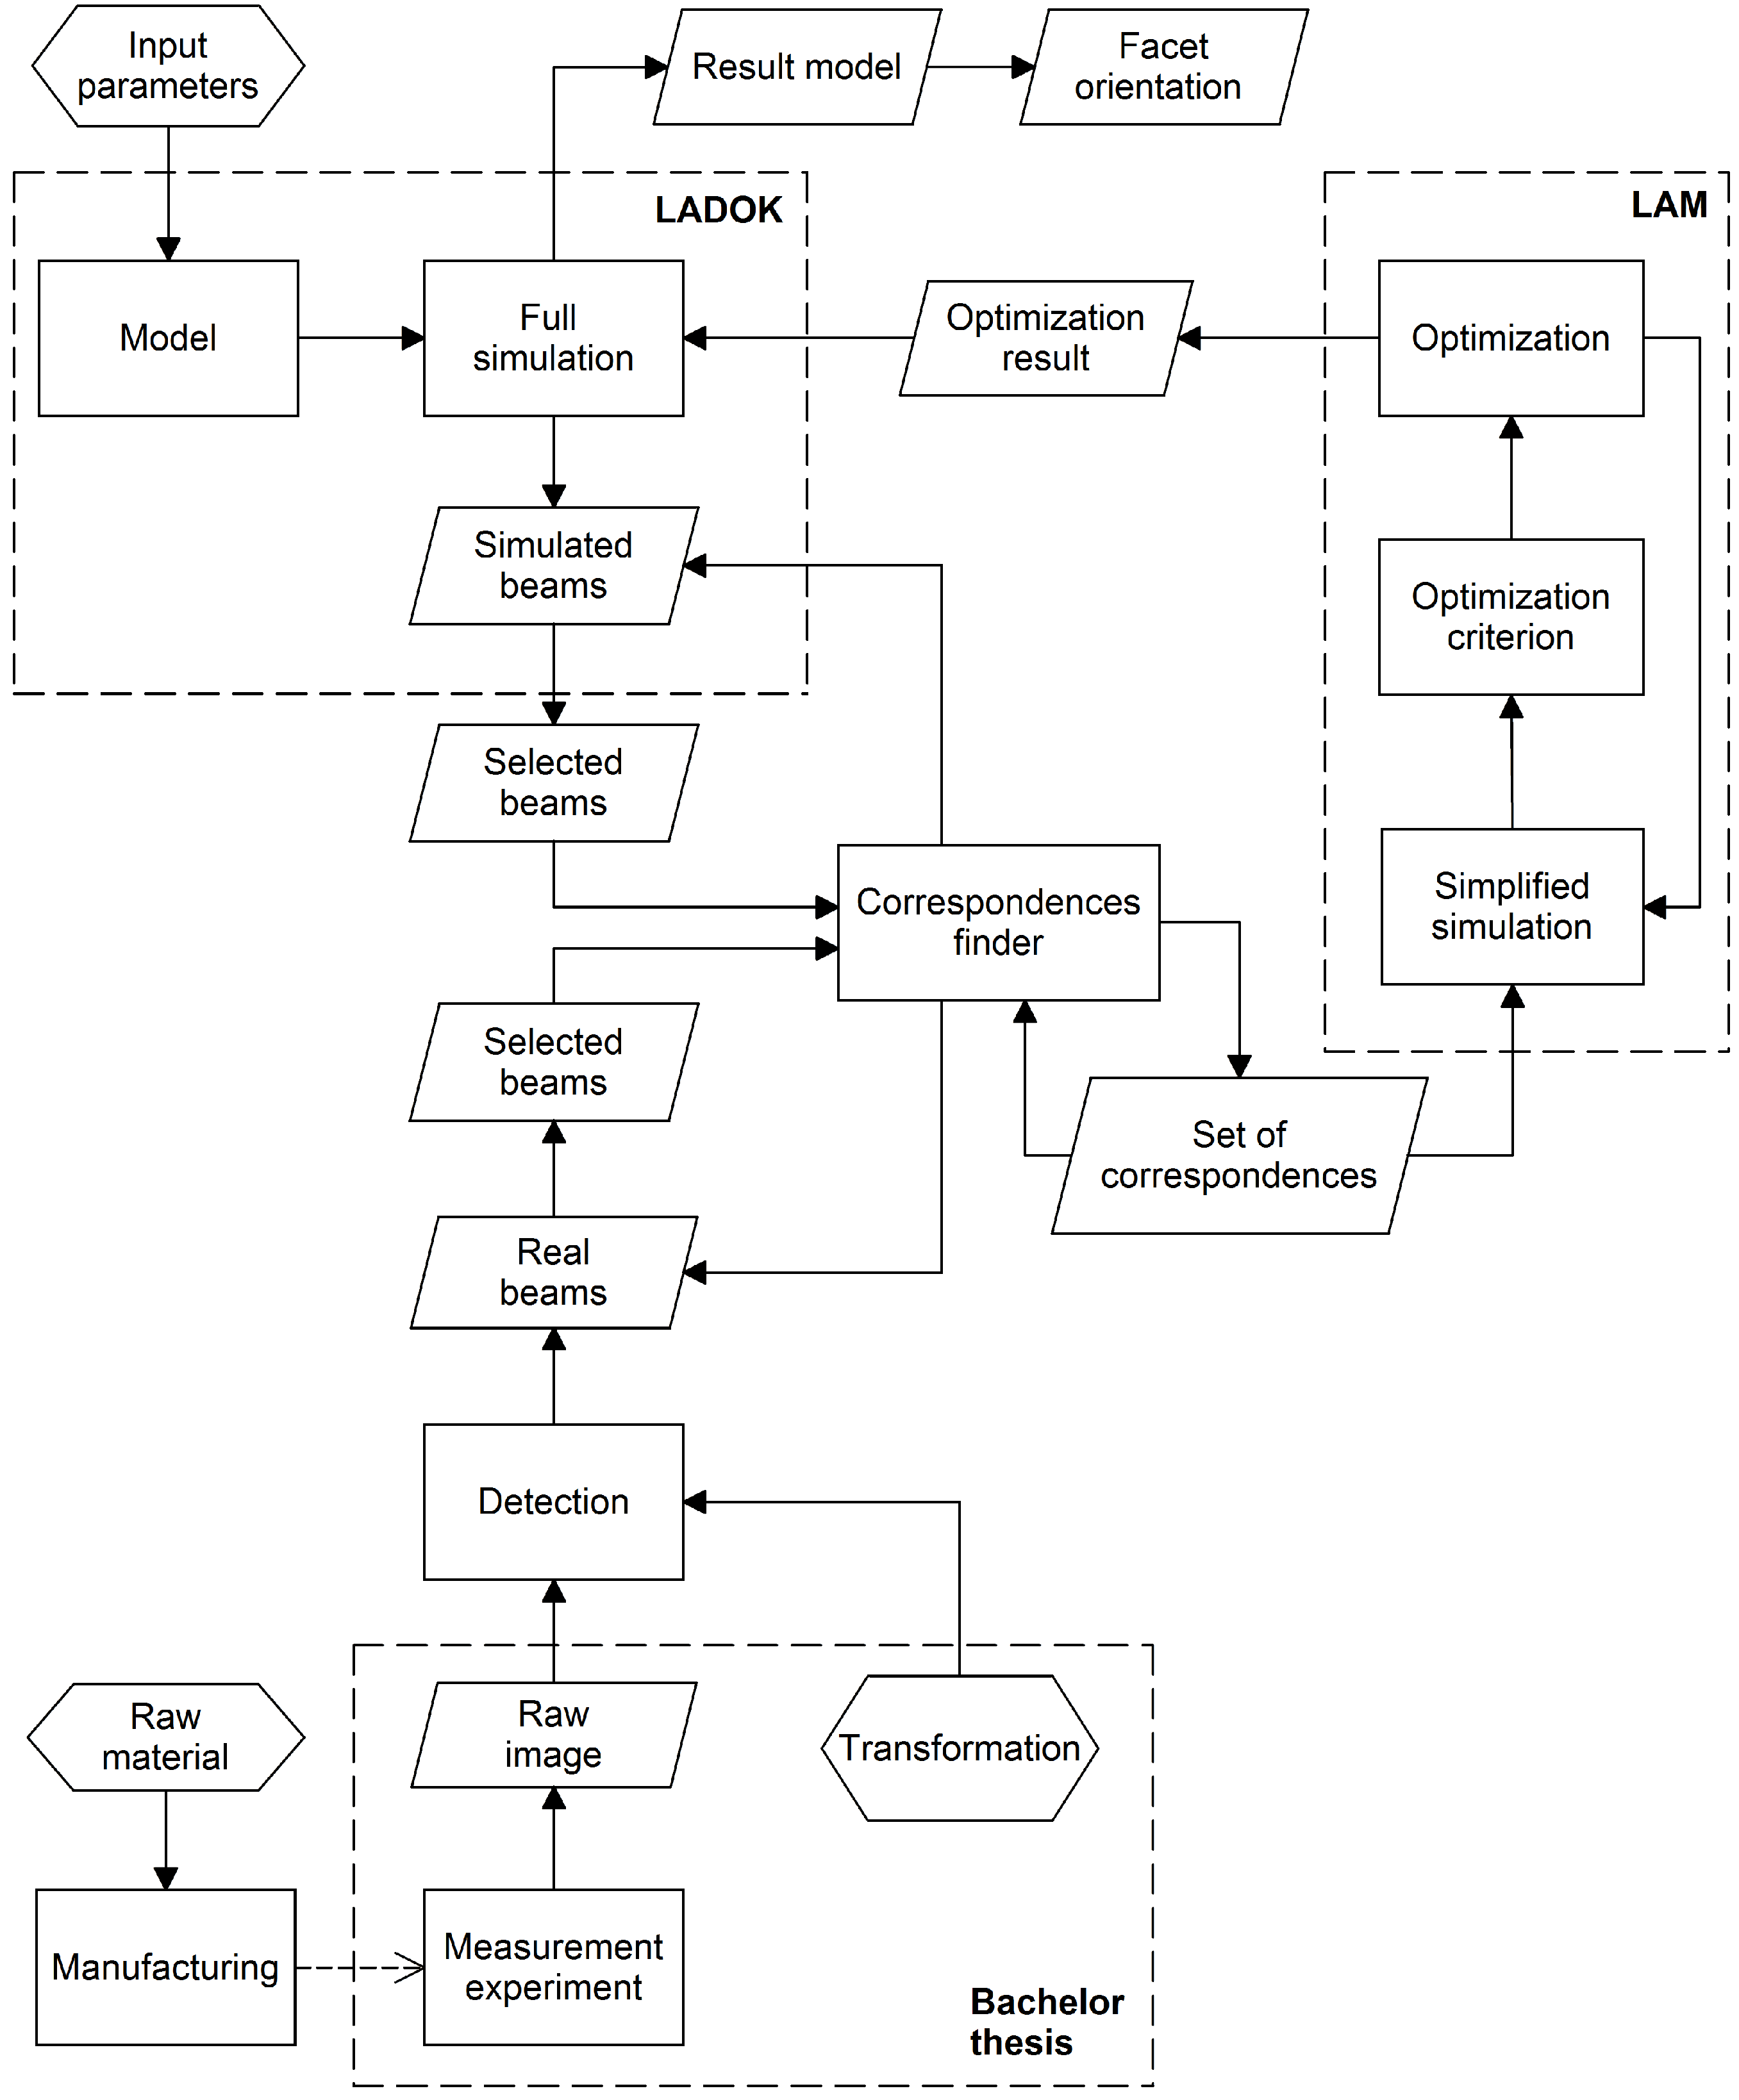
\includegraphics[width = \textwidth]{diagram.pdf}
\caption{Diagram with princip of full program.}
\label{fig:diagram}
\end{figure}


\section{Korespondence}
V nalezení korespondencí mezi simulovanými a reálnými svazky se objevuje několik komplikací. 

\section{Optimalizované kritérium}

\subsection{Podmíněnost}
Základní otázkou optimalizačního problému je, zda je systém dostatečně podmíněný. První podmínku, kterou musíme splnit je získat minimálně stejný počet nezávislých rovnic, jako je počet optimalizovaných parametrů. 

Fasety kamene modelujeme jako rovinu. Obecná má rovina čtyři stupně volnosti. Lze ji tedy jednoznačně popsat pomocí 4 parametrů tj. normálového vektoru $\vec{n} = \left[a,\,b,\,c\right]$ a vzdálenosti od souřadného systému $d$. $\vec{n}$ a $d$ máme získáme z \textit{referenčního} modelu. 

Výsledný model se oproti referenčnímu liší v parametrech faset. Změnu parametru $\vec{n}$ lze vyjádřit pomocí 
% viz str. 27
V našem případě máme optimalizujeme náklon faset.   

\section{Plná vs. zjednodušená simulace}

\section{Klasifikace příznaků}

\section{Implementace}

\section{Výsledky}

\subsection{Ruční optimalizace}

\subsection{Automatická optimalizace}

 \clearpage